\sect{Ćwiczenia 8}

\begin{frame}{Zadanie 1}
	\begin{figure}
		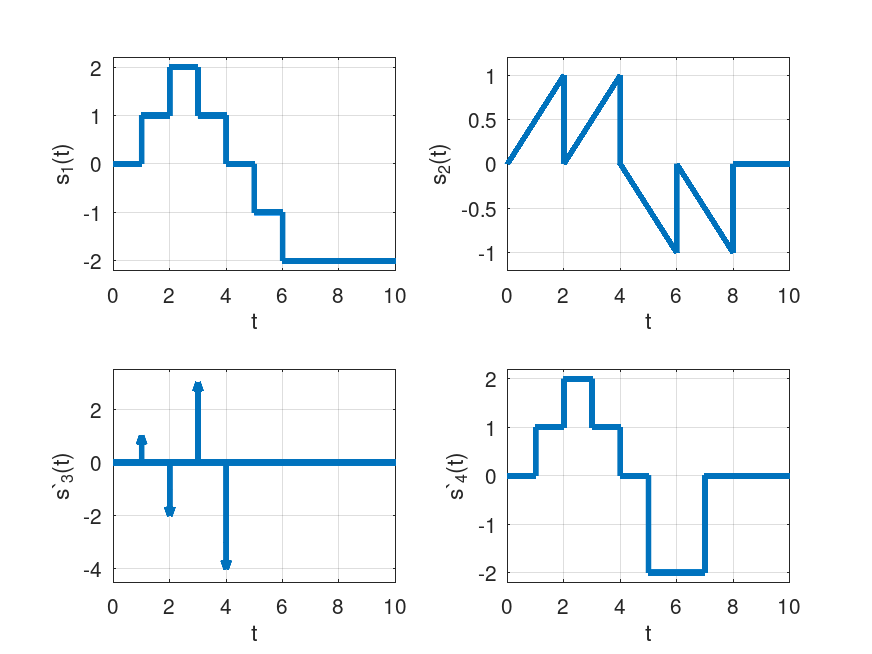
\includegraphics[scale=0.22, alt={}]{./imags/E08/ex3.png}
		\caption{Określ $s_1(t)$, $s'_1(t)$, $s_2(t)$, $s'_2(t)$, $s_3(t)$, $s'_3(t)$, $s_4(t)$, $s'_4(t)$. Narysuj $s'_1(t)$, $s'_2(t)$, $s_3(t)$, $s_4(t)$.}
	\end{figure}	
\end{frame}

\begin{frame}{Zadanie 2}
Oblicz $s'_1(t)$, $s'_2(t)$, $s_3(t)$, $s_4(t)$.\\
Narysuj $s_1(t)$, $s'_1(t)$, $s_2(t)$, $s'_2(t)$, $s_3(t)$, $s'_3(t)$, $s_4(t)$, $s'_4(t)$.
	\begin{itemize}
		\item[\bt] $s_1(t)=\mathbf{1}(t-1)-2\mathbf{1}(t-2)+\mathbf{1}(t-3)$
		\item[\bt] $s_2(t)=t\mathbf{1}(t-1)-\delta(t-2)-2t\mathbf{1}(t-3)+t\mathbf{1}(t-4)$
		\item[\bt] $s'_3(t) = \delta(t) + \delta(t-1) - 2 \delta(t-3)$
		\item[\bt] $s'_4(t) = \mathbf{1}(t-1)+\delta(t-1)-\mathbf{1}(t-2)-3\delta(t-3)$
	\end{itemize}
\end{frame} 

\begin{frame}{Zadanie 3}
Oblicz prostą transformatę Laplaca
	\begin{itemize}
		\item[\bt] $f_1(t)=5e^{-2t}$
		\item[\bt] $f_2(t)=2-2e^{-9t}$
		\item[\bt] $f_3(t)=3 sin(5t)$
		\item[\bt] $f_4(t)=4e^{-2t}sin(6t)$
		\item[\bt] $f_5(t)=t sin(10t)$
		\item[\bt] $f_6(t)=2t cos(6t)$
		\item[\bt] $f_7(t)=t e^{-3t} cos(3t)$
	\end{itemize}
\end{frame} 

\begin{frame}{Zadanie 4}
Oblicz odwrotną transformatę Laplaca
	\begin{itemize}
		\item[\bt] $f_1(s)=\frac{1}{s(s+3)}$
		\item[\bt] $f_2(s)=\frac{s}{(s+9)^2}$
		\item[\bt] $f_3(s)=\frac{s}{(s+3)(s^2+4s+29)}$
		\item[\bt] $f_4(s)=\frac{s}{(s^2+9)^2}$
	\end{itemize}
\end{frame} 